\documentclass{article}
\usepackage{geometry}
 \geometry{
 a4paper,
 total={170mm,270mm},
 left=20mm,
 top=10mm,
 }
\usepackage{graphicx}
\usepackage{float}
\usepackage{enumitem}
\usepackage{caption}
\usepackage{amsmath}
\usepackage{datetime}
\usepackage{multirow}
\usepackage{listings}

\newcommand\blfootnote[1]{%
  \begingroup
  \renewcommand\thefootnote{}\footnote{#1}%
  \addtocounter{footnote}{-1}%
  \endgroup
}
\newcommand*{\addheight}[2][.5ex]{%
  \raisebox{0pt}[\dimexpr\height+(#1)\relax]{#2}%
}
\newdate{date}{4}{10}{2016}
\date{\displaydate{date}}
\title{\textbf{Network Analysis and Modelling - CSCI 5352} \\
Problem Set 3}
\author{\textbf{Santhanakrishnan Ramani}}
\begin{document}
\maketitle

\section*{Problem 1}
\blfootnote{Collaborated with Ruhi Saraf, Irene Beckman. Discussed the values and proofs for the problems after solving all by myself.}
From Eq. (7.76) in Networks $e_{rr}$, $a_{r}$ and $Q$ are as follows,\\
$e_{rr} = \dfrac{1}{2m}\sum_{ij} A_{ij}\,\delta(c_i,r)\,\delta(c_j,r)  \texttt{ fraction of edges that join vertices of type r to vertices of type r}$\\
$a_{r} = \dfrac{1}{2m}\sum_{i} k_i\,\delta(c_i,r) \texttt{ fraction of ends of edges attached to vertices of type r}$\\
$$Q = \sum_{r} (e_{rr} - {a_r}^2)$$

Since, we are considering only the ethnicity, the table representing the fraction of edges becomes,
\begin{center}
\begin{tabular}{l r|l l l l}                      
& \multicolumn{1}{r|}{Ethnicity} &Black   &Hispanic   &White   &Other   \\ \cline{2-6}
& \multicolumn{1}{r|}{Black} &0.258   &0.014   &0.024   &0.009   \\
& \multicolumn{1}{r|}{Hispanic} &0.014   &0.157   &0.0405   &0.013   \\ 
& \multicolumn{1}{r|}{White} &0.024   &0.0405   &0.306   &0.0295   \\
& \multicolumn{1}{r|}{Other} &0.009   &0.013   &0.0295   &0.016   
\end{tabular}  
\end{center}

Since, the table values sums up to 0.997 and not 1, normalising the table we get,
\begin{center}
\begin{tabular}{l r|l l l l}                      
& \multicolumn{1}{r|}{Ethnicity} &Black   &Hispanic   &White   &Other   \\ \cline{2-6}
& \multicolumn{1}{r|}{Black} &0.2588   &0.014   &0.0241   &0.009   \\
& \multicolumn{1}{r|}{Hispanic} &0.014   &0.1575   &0.0406   &0.013   \\ 
& \multicolumn{1}{r|}{White} &0.0241   &0.0406   &0.3069   &0.0296   \\
& \multicolumn{1}{r|}{Other} &0.009   &0.0130   &0.0296   &0.016   
\end{tabular}  
\end{center}

From the definition of $e_{rr}$, we can clearly see that it is equal to the value of the fraction given in the table where both the row and column are of same type (values present in the diagonals).

\begin{table}[h!]
\centering
\begin{tabular}{ |c|c| } 
\hline
r & $e_{rr}$ \\
\hline
Black & 0.2588\\
Hispanic & 0.1575\\
White & 0.3069\\
Other & 0.016\\
\hline
\end{tabular}
\label{table:1}
\end{table}

From the definition of $a_r$, we can clearly see that it is equal to the col sum of the fraction values given in the table where the col corresponds to type r. 

\begin{table}[h!]
\centering
\begin{tabular}{ |c|c| } 
\hline
r & $a_{r}$ \\
\hline
Black & 0.3059\\
Hispanic & 0.2252\\
White & 0.4012\\
Other & 0.0677\\
\hline
\end{tabular}
\label{table:2}
\end{table}

Using the values from the tables, we get the value of modularity Q using the formula above as,  $Q = 0.4294$\\

Since the value of Q is greater than 0, we can conclude for assortative mixing or homophily in this community.
\newpage
\section*{Problem 2}
\begin{enumerate}[label=(\alph*)]
\item
To show mathematically that if we divide the undirected line graph consisting of n vertices  into any two contiguous groups, such that one group has $r$ connected vertices and the other has $n-r$, the modularity Q takes the value,
$$Q = \dfrac{3-4n+4rn-4r^2}{2(n-1)^2}$$

Since, the given network is divided into two groups, the fraction of edges starting and ending at the same group and across the two groups is given by the following table,

\begin{table}[h!]
\centering
\begin{tabular}{l r|l l}                      
& \multicolumn{1}{r|}{group} &1   &2  \\ \cline{2-4}
& \multicolumn{1}{r|}{1} &$\dfrac{r-1}{n-1}$   &$\dfrac{1}{2(n-1)}$      \\
& \multicolumn{1}{r|}{2} &$\dfrac{1}{2(n-1)}$   &$\dfrac{n-r-1}{n-1}$     
\end{tabular}
\end{table}

using the same logic as in problem and solving for $e_rr$ and $a_r$ we get the following values,

\begin{table}[H]
    \begin{minipage}{.4\textwidth}
    \centering
	\begin{tabular}{ |c|c| } 
	\hline
	r & $e_{rr}$ \\
	\hline
	&\\
	group 1 & $\dfrac{r-1}{n-1}$  \\
	group 2 & $\dfrac{n-r-1}{n-1}$\\
	\hline
	\end{tabular}
	\end{minipage}
    \begin{minipage}{.6\textwidth}
    \centering
	\begin{tabular}{ |c|c|c| } 
	\hline
	r & $a_{r}$ & ${a_r}^2$ \\
	\hline
	& &\\
	group 1 & $\dfrac{2r-1}{2(n-1)}$ & $\dfrac{4r^2-4r+1}{4(n-1)^2}$\\
	group 2 & $\dfrac{2n-2r-1}{2(n-1)}$ & $\dfrac{4n^2+4r^2+4r-4n-8rn+1}{4(n-1)^2}$\\
	\hline
	\end{tabular}
	\end{minipage}
\end{table}

Substituting the values to find Q (= $Q_1+Q_2$) we get,
$$Q_1 = Q_2 = \dfrac{3-4n+4rn-4r^2}{4(n-1)^2} \implies Q =\dfrac{3-4n+4rn-4r^2}{2(n-1)^2}$$

\item
To show that when n is even, the optimal division, in terms of modularity Q, is the division that splits the network exactly down the middle, into two parts of equal size given,

 $$Q = \dfrac{3-4n+4rn-4r^2}{2(n-1)^2}$$
Adding and subtracting $n^2$ in the numerator of the above equation we get, $$Q = \dfrac{3-4n+4rn-4r^2+n^2-n^2}{2(n-1)^2}$$
Splitting the above equation for simplification we get,
\begin{align*}
Q & = \dfrac{1+2-2n-2n+4rn-4r^2+n^2-n^2}{2(n-1)^2}\\
  & = \dfrac{(1-2n+n^2)-2(n-1)-(-4rn+4r^2+n^2)}{2(n-1)^2}\\
  & = \dfrac{(n-1)^2 - 2(n-1) -(2r-n)^2}{2(n-1)^2}\\
  & = \dfrac{(n-1)^2}{2(n-1)^2}-\dfrac{2(n-1)}{2(n-1)^2}-\dfrac{(2r-n)^2}{2(n-1)^2 }\\
\implies Q & = \dfrac{1}{2} - \dfrac{1}{n-1} - \dfrac{(2r-n)^2}{2(n-1)^2}
\end{align*}
Inorder to get the maximum value of Q using the above equation, we need to min $\frac{(2r-n)^2}{2(n-1)^2}$ as much as possible as ($\frac{1}{2} - \frac{1}{n-1}$) is constant for a given network.

Since the term $\frac{(2r-n)^2}{2(n-1)^2}$ has a square on both numerator and denominator, the only way to minimize is make the numerator equal to zero,
\begin{align*}
\implies & {(2r-n)^2} = 0\\
\implies & r = n/2
\end{align*}

Hence proved, that when n is even the optimal division, in terms of modularity Q, is the division that splits the network exactly down the middle, into two parts of equal size.
\end{enumerate}
\newpage
\section*{Problem 3}
\begin{enumerate}[label=(\roman*)]
\item
The figure below shows the plot of modularity score Q as a function of the number of merges on applying greedy agglomerative algorithm to the karate club network data.

\begin{figure}[h]
  \centering
  \begin{minipage}[b]{0.6\textwidth}
    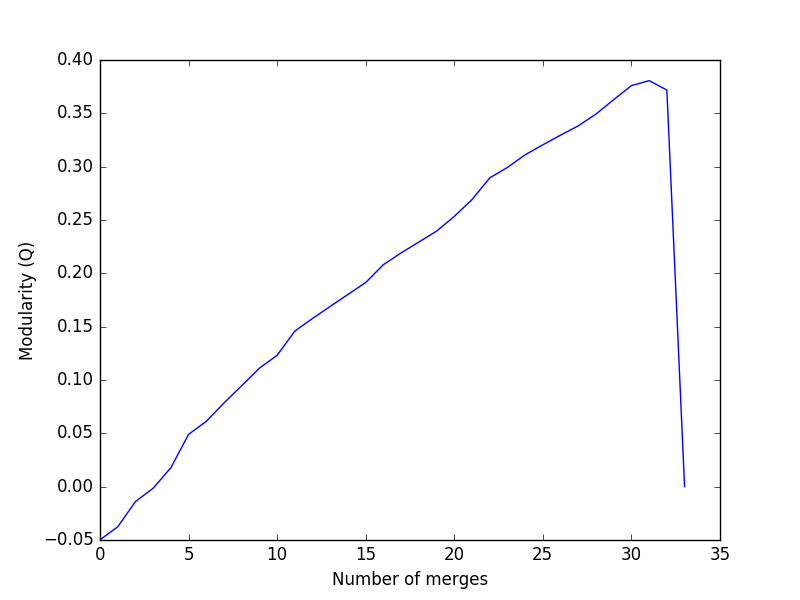
\includegraphics[width=\textwidth]{images/p3a.png}
  \end{minipage}
\end{figure}
 
\item
The figure below shows a visualization of the karate club network with vertices labelled according to the maximum modularity partition when applying the greedy agglomerative algorithm.
\begin{figure}[h]
  \centering
  \begin{minipage}[b]{0.7\textwidth}
    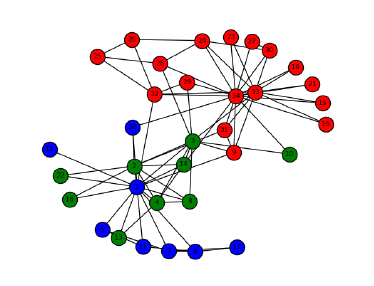
\includegraphics[width=\textwidth]{images/p3b.png}
  \end{minipage}
\end{figure}

\item
The normalized mutual information (NMI) between the partition obtained from the greedy agglomerative algorithm and the "social partition" given to us, calculated using Equation (11) in Karrer, Levina, and Newman, "Robustness of community structure in networks." is \textbf{0.5646}\\

Since the value of NMI $>$ 0.5, we can say there is some agreement although not a perfect one between the two partitions. This tells us that	 the usage of modularity maximisation to infer good partitions without knowing the labels in a network is a good, quick and easy way but not the best. The reason being the greedy agglomerative algorithm makes certain assumptions or choices at every step in order to infer the clusters as quickly as possible.

\end{enumerate}
\newpage
\section*{Problem 4}
The figure below represents the scalar plot showing the assortativity  versus network size n, on log-linear axes for each vertex attribute of all 100 networks and a density plot showing the distribution of assortativity values. The solid line in the graphs indicates no assortativity.\\

(Note: Considered the missing values as separate clusters while calculating modularity)
 
\begin{table}[H]
\centering
\begin{tabular}{|c|c|}
	\hline
	\addheight{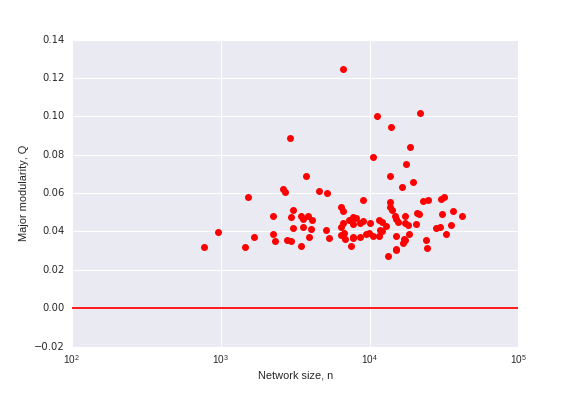
\includegraphics[width=70mm]{images/Major.png}} &
	\addheight{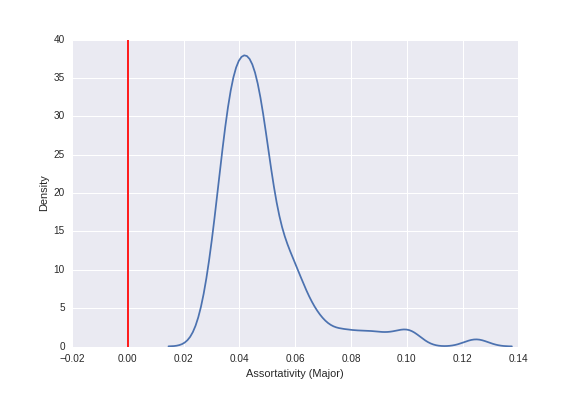
\includegraphics[width=70mm]{images/Major_density.png}} \\
	\hline   
    \addheight{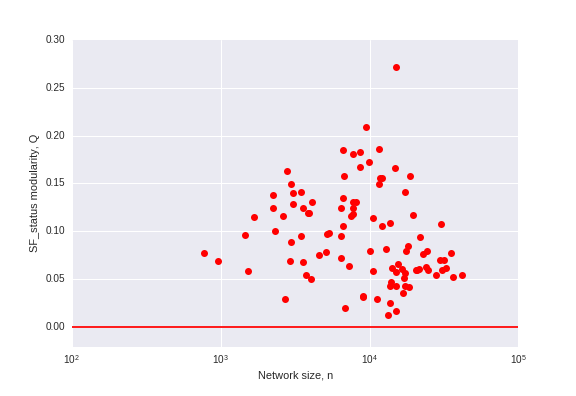
\includegraphics[width=70mm]{images/SF_status.png}} &
    \addheight{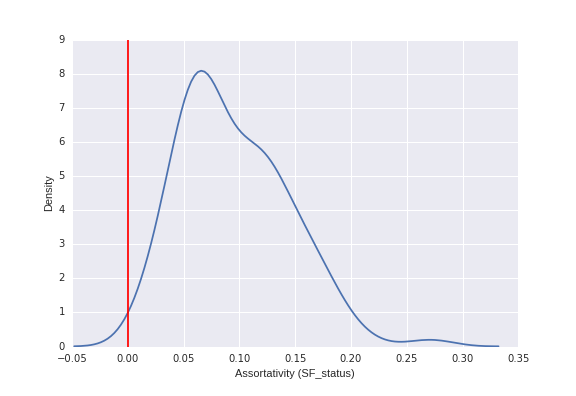
\includegraphics[width=70mm]{images/SF_status_density.png}} \\
    \hline
    \addheight{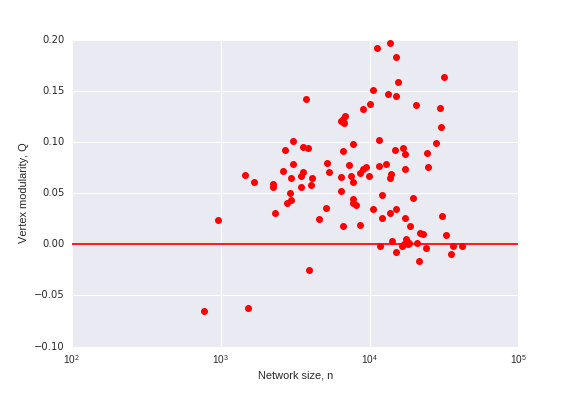
\includegraphics[width=70mm]{images/Vertex.png}} &
    \addheight{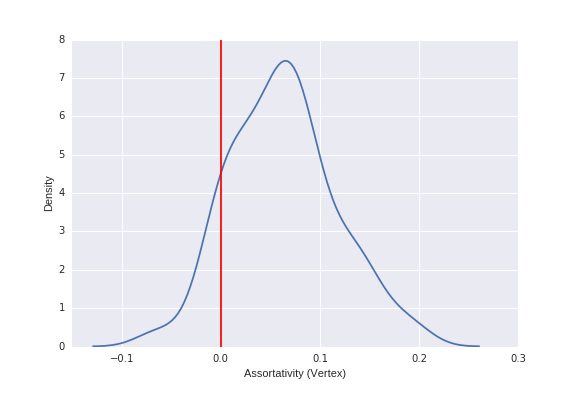
\includegraphics[width=70mm]{images/Vertex_density.png}} \\
    \hline
\end{tabular}
\end{table}

\begin{itemize}
\item
The major attribute are slightly more assortative in these social networks as all the values lie above the line of no assortivity with a mean of 0.048. The reason for this type of pattern in the facebook friendships formation can be attributed to the fact that two students in the same major are more likely to be friends than two students from different major.

\item
The Vertex degree attribute are a little more assortative in these social networks, but the values spans the no assortivity line with a mean of 0.062. The slight tendency for heterophily in this can be attributed to the fact that there will be popular or friendly students in the university who would be a friend of students having very few friends. The homophily can be attributed to the reason popular students connect to other popular students.

\item
The Student Faculty status attribute are more assortative in these social networks compared to other attributes as we can see that all the values lie above the line of no assortivity with a mean of 0.095. The reason for this type of pattern in the facebook friendships formation can be attributed to the fact that it is very highly unlikely that a student will be a friend of a faculty in facebook.
\end{itemize}
  

 
\newpage
\section*{Problem 5}
As described in Section 13.2 of Networks, the configuration model can be thought of as the ensemble of all possible matchings of edge stubs, where vertex i has $k_i$ stubs. To show that for a given degree sequence, the number $\Omega$ of matchings is independent of degree sequence.\\

Since, the sum of the degree sequence is equal to 2m (the number of stubs) where m is the no of edges. The number of combinations that can be formed using it and given as input to the configuration model is $(2m)!$.\\

The number of ways a particular edge can be formed in the configuration model is 2 as $stub_i$ can be joined to $stub_j$ or vice-versa. Since, there is total of m edges that needs to be formed, the total number of combinations is $2^m$. And, the number of combinations by which the same list of edges can be formed by the configuration model is $m!$ as there are m edges.\\

So the total number of matchings is given by the fraction of total number of combinations $2m!$ by the no of ways the same edge could be formed multiplied by the number of combinations of the same edge list ($2^m m!$) which is independent of the degree sequence.

$$ \Omega = \dfrac{(2m)!}{2^m m!}$$ 
 
\section*{Problem 6}
\begin{itemize}
\item
The mean fractional size of the largest component for a network with n = $10^4$ vertices, and with $p_1$ = 0.6, $p_3$ = $1-p_1$, and $p_k$ = 0 for all other values of k(degree of a vertex) calculated via computer simulation is \textbf{0.633924}.
\item
The figure below shows the mean fractional size of the largest component of a network of size $10^4$ with values of $p_1$ from 0 to 1 in steps of 0.01 formed using the configuration model and averaged over 2000 configurations for every value of $p_1$.\\
\begin{figure}[H]
  \centering
  \begin{minipage}[b]{0.6\textwidth}
    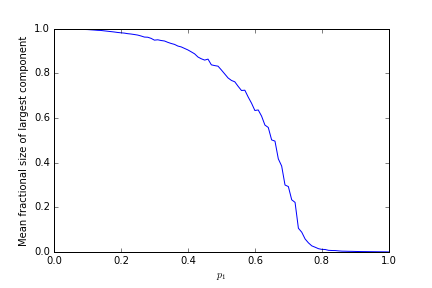
\includegraphics[width=\textwidth]{images/p6.png}
  \end{minipage}
\end{figure}
From the figure above, we can clearly see that the mean fractional size of largest component starts  decreasing as we increase the value of $p_1$ from 0 to 1 in steps of 0.01, and it starts to disappears when $p_1 \geq 0.8$. This allows us to estimate the value of p1 for the phase transition at which the giant component disappears.  
\end{itemize}
\newpage
\section*{Code for Problem 3}
\begin{lstlisting}[language=Python, breaklines=true]
import networkx as nx
import numpy as np
from collections import defaultdict
import matplotlib.pyplot as plt
from sklearn import metrics
import math
import collections

def NMI( labels_pred, labels_true ):
    V = len(labels_pred)
    C = set(labels_pred)
    Cdash = set(labels_true)
    Ci = defaultdict(int)
    Cdashj = defaultdict(int)
    
    HC = 0
    for i in C:
        Ci[i] = len([1 for j in labels_pred if j == i])
        HC += ((float(Ci[i])/V) * math.log(float(Ci[i])/V))
    
    HCdash = 0
    for i in Cdash:
        Cdashj[i] = len([1 for j in labels_true if j == i])
        HCdash += ((float(Cdashj[i])/V) * math.log(float(Cdashj[i])/V))
    
    merge = zip(labels_pred, labels_true)
    ICCdash = 0
    for i in C:
        for j in Cdash:
            intersect = len([1 for (u,v) in merge if (u == i and v == j)])
            if intersect != 0:
                ICCdash += ((float(intersect)/V) * math.log((float(intersect) * V)/(Ci[i] * Cdashj[j])) )
    
    return (-2.0 * ICCdash) / (HC + HCdash)

def geteuv(edges, group_u, group_v):
    sum = 0
    for x,y in edges:
        if (x in group_u and y in group_v) or (x in group_v and y in group_u):
            if (group_u == group_v):
                sum = sum + 2
            else:
                sum = sum + 1
    return sum/(2.0*len(edges))

fileName = "/home/santa/Dropbox/NAM/Problem Set 3/Data/karate_club_edges.txt"
lines = [line.rstrip('\n') for line in open(fileName)]
edges = []
for line in lines:
    edges.append((int(line.split()[0]),int(line.split()[1])))
G = nx.Graph()
G.add_edges_from(edges)
sum = 0   
for node in G.nodes():
    sum = sum + (G.degree(node)**2)
Q = (-1.0/(4.0*(G.number_of_edges()**2))) * sum

groups = {}
for i in range(1,G.number_of_nodes()+1):
    groups[i] = range(i,i+1)

qList = []
qList.append(Q)
while len(groups) > 1:
    
    e = np.zeros((G.number_of_nodes()+1,G.number_of_nodes()+1))
    for u in groups:
        for v in groups:
            e[u][v] = geteuv(edges, groups[u], groups[v])

    delQ = -10
    dQ = np.zeros((len(groups)+1,len(groups)+1))
    for i in range(len(groups)):
        for j in range(i+1,len(groups)):
            u = groups.keys()[i]
            v = groups.keys()[j]
            temp = 2 * (e[u][v] - (e[:,u].sum() * e[:,v].sum()))
            dQ[i][j] = temp
            if temp > delQ:
                delQ = temp
                maxu, maxv = u,v
    if Q > Q+delQ:
        break
    groups[maxu] = groups[maxu] + groups[maxv]
    groups.pop(maxv,None)
    Q = Q+delQ
    qList.append(Q)

groups_labels = {}
club_labels = {}
i = 0
for k,v in groups.iteritems():
    i = i+1
    for l in v:
        groups_labels[l] = l
        club_labels[l] = i

plt.plot(qList)
plt.xlabel('Number of merges')
plt.ylabel('Modularity (Q)')
plt.show()
pos = nx.fruchterman_reingold_layout(G)
nx.draw_networkx_nodes(G,pos,nodelist=groups[1], node_color='b')
nx.draw_networkx_nodes(G,pos,nodelist=groups[2], node_color='g')
nx.draw_networkx_nodes(G,pos,nodelist=groups[9], node_color='r')
nx.draw_networkx_edges(G,pos,edgelist=edges)
nx.draw_networkx_labels(G,pos,groups_labels,font_size=8)
plt.show()

file = open("/home/santa/Dropbox/NAM/Problem Set 3/Data/karate_club_edges_predict.txt", "w")
club_labels = collections.OrderedDict(sorted(club_labels.items()))
list_pred = []
for k in club_labels:
    list_pred.append(int(club_labels[k]))
    file.write(str(k) + "\t" + str(club_labels[k]) + "\n")
file.close()

fileName = "/home/santa/Dropbox/NAM/Problem Set 3/Data/karate_club_labels.txt"
lines = [line.rstrip('\n') for line in open(fileName)]
list_true = []
for line in lines:
    list_true.append(int(line.split()[1]))

print NMI(list_pred, list_true)
\end{lstlisting}
\newpage
\section*{Code for Problem 4}
\begin{lstlisting}[language=Python, breaklines=true]
import os
import re
import networkx as nx
from collections import defaultdict

def modularity(edges, groups, attribute):
    e = np.zeros((len(attribute),len(attribute)))
    for edge in edges:
        u = attribute.index(int(groups[edge[0]]))
        v = attribute.index(int(groups[edge[1]]))
        e[u][v] += 1
    for row in range(len(attribute)):
        for col in range(len(attribute)):
            e[row][col] = e[row][col] / (1.0 * len(edges))
    ai = ei =0
    for i in range(len(attribute)):
        ai = ai + e[i].sum()**2
        ei = ei + e[i][i]
    return ei - ai

def vertexDegree(matrix, no_of_edges, degree, nodes):
    num = den = 0
    for i in range(len(nodes)):
        xi = degree[i]
        for j in range(i,len(nodes)):
            xj = degree[j]
            prod = (xi*xj)
            temp = (prod)/(2.0*no_of_edges)
            if i==j:
                den += ((xi - temp)*prod)
                num -= (prod * temp)
            else:
                den -= (2.0 * temp * prod) 
                num += (2.0 * prod * (matrix[i,j] - temp))
    return (num/den)

dataPath = "/home/santa/Dropbox/NAM/Problem Set 3/Data/facebook100txt/"
for filename in os.listdir(dataPath):
    if filename.endswith(".txt") and not filename.endswith("attr.txt") and filename.find("readme") == -1:
        print filename
        lines = [line.rstrip('\n') for line in open(dataPath+filename)]
        edges = []
        nodes = set()
        for line in lines:
            vertexes = line.split("\t")
            x,y = int(vertexes[0]), int(vertexes[1])
            nodes.add(x)
            nodes.add(y)
            edges.append((x,y))
        
        G = nx.Graph()
        G.add_edges_from(edges)
        G.add_nodes_from(nodes)
        degree = list(G.degree(G.nodes()).values())
        matrix = nx.adjacency_matrix(G)
        matrix = matrix.todense()

        attr_filename = filename.replace(".txt","_attr.txt")
        lines = [line.rstrip('\n') for line in open(dataPath+attr_filename)]
        lines.pop(0)
        major = defaultdict(list)
        majorSet = set()
        sfstatus = defaultdict(list)
        sfstatusSet = set()
        for line in lines:
            values = line.split("\t")
            sfstatusSet.add(int(values[1]))
            sfstatus[int(values[0])] = int(values[1])
            majorSet.add(int(values[3]))
            major[int(values[0])] = int(values[3])
        
        name = filename[:re.search("\d", filename).start()]
        file = open("/home/santa/Dropbox/NAM/Problem Set 3/Code/prob4.txt", "a")
        file.write(name + "," + str(len(nodes)) + "," + str(modularity(edges, sfstatus, list(sfstatusSet))) + "," + str(modularity(edges, major, list(majorSet))) + "," + str(vertexDegree(matrix, G.number_of_edges(), degree, nodes)) + "\n")
        file.close()
\end{lstlisting}

\begin{lstlisting}[language=Python, breaklines=true, caption=To plot the graphs]      
import matplotlib.pyplot as plt
import pandas as pd
import numpy as np
import seaborn as sns

csv_file = "/home/santa/Dropbox/NAM/Problem Set 3/Code/prob4.csv"
df = pd.read_csv(csv_file)
lst = ['Major', 'SF_status', 'Vertex']
for item in lst:
    x = df['Size'].tolist()
    y = df[item].tolist()
    plt.plot( x, y, 'ro')
    plt.axhline( y=0,  color='r')
    plt.xscale('log')
    plt.xlabel('Network size, n')
    plt.ylabel(item + ' modularity, Q')
    plt.savefig("/home/santa/Dropbox/NAM/Problem Set 3/Latex/images/"+ item+".png")
    plt.clf()
    sns.kdeplot( np.array( y ) )
    plt.axvline( x=0, color='r' )
    plt.xlabel('Assortativity (' + item + ')')
    plt.ylabel('Density')
    plt.savefig("/home/santa/Dropbox/NAM/Problem Set 3/Latex/images/"+ item+"_density.png" )
    plt.clf()
\end{lstlisting}
\newpage
\section*{Code for Problem 6}
\begin{lstlisting}[language=Python, breaklines=true]
import networkx as nx
import random

for p in range(0,101,1):
    size = 0
    degreeSeq = []
    noOfNodes = 10000
    for i in range(noOfNodes):
        if random.uniform(0, 1) <= (float(p)/100):
            degreeSeq.append(int(1))
        else:
            degreeSeq.append(int(3))
    
    vector = []
    for i in range(len(degreeSeq)):
       for j in range(degreeSeq[i]):
           vector.append(i)
    
    noOfIter = 2000
    for i in range(noOfIter):
        random.shuffle(vector)
        edges = []
        for a,b in zip(vector[0:][::2],vector[1:][::2]):
            edges.append((a,b))
        G = nx.Graph()
        G.add_edges_from(edges)
        G.remove_edges_from(G.selfloop_edges())
        G.add_nodes_from(range(noOfNodes))
        Gcc=sorted(nx.connected_component_subgraphs(G), key = len, reverse=True)
        G0=Gcc[0]
        size += float(G0.number_of_nodes())/10000
    
    file = open("/home/santa/Dropbox/NAM/Problem Set 3/Code/prob6_2.txt", "a")
    file.write(str((float(p)/100)) + "," + str(size/noOfIter) + "\n")
    file.close()
\end{lstlisting}
\begin{lstlisting}[language=Python, breaklines=true, caption=To plot the graph]
import matplotlib.pyplot as plt
import pandas as pd

csv_file = "/home/santa/Dropbox/NAM/Problem Set 3/Code/prob6_2.csv"
df = pd.read_csv(csv_file)
y = df['size'].tolist()
x = df['p1'].tolist()

plt.plot( x, y)
plt.xlabel(r'$p_1$')
plt.ylabel('Mean fractional size of largest component')
plt.savefig("/home/santa/Dropbox/NAM/Problem Set 3/Latex/images/p6.png")
plt.clf()
\end{lstlisting}
\end{document}
